%%%%%%%%%%%%%%%%%%%%%%%%%%%%%%%%%%%%%%%%%%%%%%%%%%%%%%%%%%%%%%%%%%%%%
%% Copyright 2020 Mike Jones, <dr.mike.jones@gmail.com>
%% AKA Grey Wolf <mike.jones@mansouthscouts.org>
%% [23rd Manchester (Birch with Fallowfield)]
%% Scout Membership number: 12114313
%
% This file is part of Grey Wolf's Scouts Beamer Theme.
%
% Grey Wolf's Scouts Beamer Theme is free software: you can redistribute
% it and/or modify it under the terms of the GNU General Public License
% as published by the Free Software Foundation, either version 3 of the
% License, or (at your option) any later version.
%
% Grey Wolf's Scouts Beamer Theme is distributed in the hope that it will 
% be useful, but WITHOUT ANY WARRANTY; without even the implied warranty
% of MERCHANTABILITY or FITNESS FOR A PARTICULAR PURPOSE.  See the GNU
% General Public License for more details.
%
% You should have received a copy of the GNU General Public License
% along with Grey Wolf's Scouts Beamer Theme.  If not, see
% <https://www.gnu.org/licenses/>.
%%%%%%%%%%%%%%%%%%%%%%%%%%%%%%%%%%%%%%%%%%%%%%%%%%%%%%%%%%%%%%%%%%%%%

%stacked logo slide
\logoslide[noheadlogo,type=stacked]

%Front Cover
\logoslide[noheadlogo]
%\logoslide[noheadlogo,text=23rd Manchester \\ (Birch with Fallowfield)]

%Big logo slide (no header)
\logoslide[noheadlogo,type=fleur-de-lis]

%Big Teal logo slide
\changecolours[logo=purple]{ScoutTeal}
\logoslide[type=fleur-de-lis]

%TitlePage Purple
\changecolours[inverse]{ScoutPurple}
\frame[plain]{\titlepage}

%TitlePage with BG1
{
\bgimage{media/image1}
\begin{frame}[plain]
\titlepage
\end{frame}
}

%TitlePage with BG2
{
\bgimage[position=f,gravity=C]{media/image2}
\begin{frame}[plain]
\titlepage
\end{frame}
}

%A a table of contents perhaps:
%\begin{frame}[allowframebreaks]{Outline}\tableofcontents\end{frame}

%Section Slides - These create divider slides and TOC entries and change the current section label (for subsequent slides)
\changecolours{ScoutTeal}
\section*{Divider With * eg (\textbackslash section)}%Optional * means that this Section divider slide is omitted.
\subsection{Subhead goes here (\textbackslash subsection)}

\changecolours{ScoutRed}
\section*{Divider Example again (\textbackslash section)}
\subsection{Subhead goes here (\textbackslash subsection)}

\changecolours{ScoutGreen}
\subsection{Subhead goes here (\textbackslash subsection)}

\changecolours{ScoutBlue}
\subsection{Subhead goes here (\textbackslash subsection)}

%A balanced two part slide
\changecolours[logo=ScoutBlack,inverse]{ScoutBlue}
{
\bgimage[position=r,gravity=E]{media/image3}
\twocolframe{%

\vspace{-0.4\baselineskip}% Just mucking about with vertical space here!
Be part of something amazing.\linebreak
Put your skills to use and learn new ones.
Give young people the skills they need to succeed in life
and discover how being a part of the Scouting family can be as rewarding for you as it is for them.
\par\vspace{\baselineskip}\par
\alert{\#SkillsForLife}\par\alert{\href{https://scouts.org.uk/join}{scouts.org.uk/join}}
}{}%
}

\changecolours[head=ScoutBlack,inverse]{ScoutPurple}
{
\bgimage[position=l,gravity=W]{media/image4}
\twocolframe{}{%

\vspace{-0.4\baselineskip}% Just mucking about with vertical space here!
Be part of something amazing.\linebreak
Put your skills to use and learn new ones.
Give young people the skills they need to succeed in life
and discover how being a part of the Scouting family can be as rewarding for you as it is for them.
\par\vspace{\baselineskip}\par
\alert{\#SkillsForLife}\par\alert{\href{https://scouts.org.uk/join}{scouts.org.uk/join}}
}%
}

%All subsequent slided lose their title text in header.
\headervisibility[hideheadtext]

\changecolours[head=ScoutBlack,inverse]{ScoutRed}
{
\bgimage[position=l,gravity=W]{media/image5}
\twocolframe{}{%

\vspace{-0.4\baselineskip}% Just mucking about with vertical space here!
Be part of something amazing.\\
Put your skills to use and learn new ones.
Give young people the skills they need to succeed in life
and discover how being a part of the Scouting family can be as rewarding for you as it is for them.
\par\vspace{\baselineskip}\par
\alert{\#SkillsForLife}\par\alert{\href{https://scouts.org.uk/join}{scouts.org.uk/join}}
}%
}

\changecolours[head=ScoutBlack,inverse]{ScoutGreen}
{
\bgimage[position=l,gravity=W]{media/image6}
\twocolframe{}{%

\vspace{-0.4\baselineskip}% Just mucking about with vertical space here!
Be part of something amazing.\\
Put your skills to use and learn new ones.
Give young people the skills they need to succeed in life
and discover how being a part of the Scouting family can be as rewarding for you as it is for them.
\par\vspace{\baselineskip}\par
\alert{\#SkillsForLife}\par\alert{\href{https://scouts.org.uk/join}{scouts.org.uk/join}}
}%
}


\changecolours[logo=ScoutBlack]{ScoutPurple}
{
\bgimage[position=r,gravity=E]{media/image7}
\twocolframe{%

\vspace{-0.4\baselineskip}% Just mucking about with vertical space here!
Be part of something amazing.\\
Put your skills to use and learn new ones.
Give young people the skills they need to succeed in life
and discover how being a part of the Scouting family can be as rewarding for you as it is for them.
\par\vspace{\baselineskip}\par
\alert{\#SkillsForLife}\par\alert{\href{https://scouts.org.uk/join}{scouts.org.uk/join}}
}{}%
}

{
\bgimage[position=r,gravity=E]{media/image7}
\twocolframe{%
\setbeamertemplate{items}{\tiny\raisebox{0.5ex}{\textbullet}}%

\vspace{-0.4\baselineskip}% Just mucking about with vertical space here!
\alert{Skills For Life}\\
Scouting gives young people the skills to succeed. These include:
\itemseps[topsepi=5mm,itemsepi=4.5mm,labelsep=0mm,leftmargini=2.5mm]
\begin{itemize}
\item{Character skills like resillience, initiative, independence and tenacity}
\item{Employability skills like leadership, teamwork, and problem solving}
\item{Practical skills lie coding, cookind and First Aid.}
\end{itemize}
}{}%
}

\changecolours{ScoutPurple}
{
\bgimage[position=l,gravity=W]{media/image8}
\twocolframe[leftcol=5.6cm]{}{%

\vspace{-0.4\baselineskip}% Just mucking about with vertical space here!
Be part of something amazing.\\
Put your skills to use and learn new ones.
Give young people the skills they need to succeed in life
and discover how being a part of the Scouting family can be as rewarding for you as it is for them.
\par\vspace{\baselineskip}\par
\alert{\#SkillsForLife}\par\alert{\href{https://scouts.org.uk/join}{scouts.org.uk/join}}
}%
}

\changecolours[text=ScoutBlack]{ScoutPurple}
\frame{%
\frametitle{Skills For Life}%
\vspace{-\baselineskip}% Sometimes you just need to remove some space.
Scouting gives young people the skills to succeed. These include:
\itemseps[topsepi=2mm,itemsepi=4.3mm,labelsep=2.9mm,leftmargini=5mm]
\begin{itemize} 
\item{Character skills like resillience, initiative, independence and tenacity}
\item{Employability skills like leadership, teamwork, and problem solving}
\item{Practical skills like coding, cookind and First Aid.}
\end{itemize}
}

\begin{frame}
\vspace{6mm}
As Scouts, we believe in preparing young people with skills
for life.
\vspace{0.35\baselineskip}

That’s why we encourage our young people to do more,
learn more and be more.
\vspace{0.35\baselineskip}

Each week, we help over 460,000 young people enjoy fun
and adventure while developing the skills they need to
succeed in life. We’re talking teamwork, leadership and
resilience: the skills that make all the difference.

\vspace{0.35\baselineskip}
\alert{\fontseries{ub}\selectfont\#SkillsForLife}\linebreak
\alert{\href{https://scouts.org.uk}{scouts.org.uk}}
\end{frame}

\changecolours[inverse]{ScoutPurple}
\begin{frame}
\frametitle{Welcome}
\begin{minipage}[t]{1.1\textwidth}% like a box a bit wider than the nominal textwidth set by having 2.8cm margins in preamble
\raggedright% force left aligned text instead of justified (to fit Scouts PPT template better)
We’re so proud to share our brand with you. This guide will
help you understand who we are, what\\
we do and how we present ourselves to the world. Please
use our brand with pride and treat it with respect. When we
have a strong, unified and consistent brand, making our
benefits clear we will attract more support for Scouting.
\end{minipage}
\end{frame}

\frame{%
\frametitle{Skills For Life}
\vspace{-\baselineskip}% Sometimes you just need to remove some space.
\begin{minipage}[t]{1.05\textwidth}% like a box a bit wider than the nominal textwidth set by having 2.8cm margins in preamble
\raggedright% force left aligned text instead of justified (to fit Scouts PPT template better)
Scouting gives young people the skills to succeed. These include:
%\itemindents{2mm}{4mm}{4mm}{4mm}
%\itemseps{4mm}{4.5mm}{}{}
\itemseps[topsepi=4mm,itemsepi=4.5mm,labelsep=2mm,leftmargini=4mm]
\begin{itemize}
\item{Character skills like resillience, initiative, independence and tenacity}
\item{Employability skills like leadership, teamwork, and problem solving}
\item{Practical skills like coding, cookind and First Aid.}
\end{itemize}
\end{minipage}
}

\changecolours[text=ScoutBlack]{ScoutPurple}
\begin{frame}
\hspace*{1mm}
\begin{minipage}[t]{0.95\textwidth}
\raggedright
\vspace*{2mm}
\begin{multicols}{2}
\footnotesize % there's no point trying to be exact here as O365 doesn't even honour the Nunito Sans font (look at the g's)
\linespread{1.1}\selectfont
As Scouts, we believe in preparing
young people with skills for life. 
\par
\vspace{\baselineskip}
That’s why we encourage our young
people to do more, learn more and be
more. Each week, we help over
460,000 young people enjoy fun and
adventure while developing the skills
they need to succeed. We’re talking
about teamwork, leadership and
resilience: the skills that make all the
difference.
\par
\vspace{2\baselineskip}
These skills have helped Scouts
become astronauts and Olympians, but
teachers and social workers too.
\par
\vspace{\baselineskip}
We believe in bringing people together
and helping them feel part of
something bigger. We celebrate
difference and stand against
intolerance, always. We’re a worldwide
force for good, creating stronger
communities and inspiring positive
futures.
\par
\vspace{\baselineskip}
\alert{\#SkillsForLife}

\end{multicols}
\end{minipage}
\end{frame}

\begin{frame}
% More tweeks with minipage follow, if you want to get reallyClose(TM), 
% but really it's not consistant so better off just using the template without!
% O365 breaks the font again: WYSI_N_WYG, grrrr!
\hspace*{1mm}
\begin{minipage}[t]{0.95\textwidth}
\raggedright
\vspace*{1mm}
\begin{multicols}{3}
%More tweeks for the emphasised purple column
\begin{minipage}[t]{\columnwidth}
\vspace{-1mm} 
\scriptsize
\raggedright
\linespread{1.2}\selectfont
\alert{Lorem ipsum dolor sit
amet, consectetur
adipiscing text elit.
Pellentesque vesti
bulum eu nibh eget
pellentesque.}
\end{minipage}
\vfill
\columnbreak
\tiny
Lorem ipsum dolor sit amet,
consectetur adipiscing elit.
Pellentesque vestibulum eu nibh
eget pellentesque. Donec egestas
risus eget mauris ultricies
scelerisque. Donec massa felis,
faucibus congue varius sit amet,
varius eget mi.\\
Donec commodo tortor quis
metus congue, eget lacinia eros
pharetra. Ut feugiat rhoncus
tincidunt. Morbi et ullamcorper
nisl. Donec commodo tortor quis
metus congue, eget lacinia eros
pharetra. Ut feugiat rhoncus
tincidunt. Morbi et ullamcorper
nisl.

Donec massa felis, faucibus
congue varius sit amet, varius
eget mi. Donec commodo tortor
quis metus congue, eget lacinia
eros pharetra. Ut feugiat rhoncus
tincidunt. Morbi et ullamcorper
nisl. Aenean bibendum tempus
congue. Vivamus suscipit
tincidunt lorem gravida tempor.
Curabitur ultricies consectetur
fermentum.\\
Maecenas fringilla ac nulla id
maximus. Suspendisse dictum
lectus et gravida interdum.
Praesent facilisis tortor a leo
ornare, eu vulputate massa.

\end{multicols}
\end{minipage}
\end{frame}

\begin{frame}
% More tweeks with minipage follow, if you want to get reallyClose(TM), 
% but really it's not consistant so better off just using the template without!
% O365 breaks the font again: WYSI_N_WYG, grrrr!
\hfill%
\begin{minipage}[t]{0.95\textwidth}
\raggedright
\vspace*{3mm}
\setlength{\columnsep}{2mm}
\begin{multicols}{4}
\Tiny
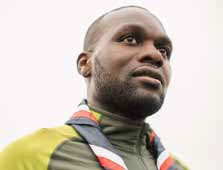
\includegraphics[height=1.5cm]{media/image10}
\par
\vspace{1.4mm}
\fontseries{eb}\linespread{1.2}\selectfont Dwayne Fields\\Scout Ambassador
\par
\vspace{1.2\baselineskip}
\begin{minipage}[t]{\columnwidth}
\fontseries{m}\linespread{1.4}\selectfont
\raggedright
Dwayne is a polar explorer
and speaker. He is the first
black Briton to reach the
North Pole, and only the
second black man in the
world to achieve this feat.
Born in Jamaica, he grew up
in Hackney, London.
\end{minipage}
\vfill
\columnbreak

\includegraphics[height=1.5cm]{media/image11}
\par
\vspace{1.4mm}
\fontseries{eb}\linespread{1.2}\selectfont Helen Glover\\Scout Ambassador
\par
\vspace{1.2\baselineskip}
\begin{minipage}[t]{\columnwidth}
\fontseries{m}\linespread{1.4}\selectfont
\raggedright
Helen is a two-time Olympic
champion and triple World
Champion, winning British
women’s rowing’s first ever
gold medal at London 2012.
\end{minipage}
\vfill
\columnbreak

\includegraphics[height=1.5cm]{media/image9}
\par
\vspace{1.4mm}
\fontseries{eb}\linespread{1.2}\selectfont Tim Peake\\Scout Ambassador
\par
\vspace{1.2\baselineskip}
\begin{minipage}[t]{\columnwidth}
\fontseries{m}\linespread{1.4}\selectfont
\raggedright
ESA Astronaut Major Tim
Peake is also a former Cub
Scout and an advocate of the
power of Scouting to help
young people develop skills
for life.
\end{minipage}
\vfill
\columnbreak
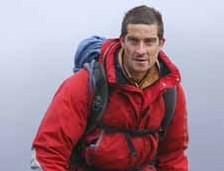
\includegraphics[height=1.5cm]{media/image12}
\par
\vspace{1.4mm}
\fontseries{eb}\linespread{1.2}\selectfont Bear Grylls\\Chief Scout
\par
\vspace{1.2\baselineskip}
\begin{minipage}[t]{\columnwidth}
\fontseries{m}\linespread{1.4}\selectfont
\raggedright
Bear was appointed in 2009
as the youngest ever Chief
Scout of the United Kingdom.
He has inspired hundreds of
thousands of young people
with his positivity, passion for
adventure, courage and
leadership.
\end{minipage}
\vfill
\end{multicols}
\end{minipage}
\hfill
\end{frame}

\changecolours{ScoutPurple}
\section{Thank you}